\documentclass[10pt]{article}
\usepackage[margin=0.8in]{geometry}
\usepackage[T1]{fontenc}
\usepackage{graphicx}
\begin{document}
\section*{Koblitz n23, m=3--15: fixed enumeration wave}
All 26 frozen native cells have terminal restricted S3 custody. The same
public field, curve, generator and target were used at every arity within
each twist. Both twists at m3 and m4 completed and verified exhaustive
fixed-factor-base negatives. Both twists at every m5--15 reached the
frozen 30-second native cap; those results are censored. No PDP witness or
independently recovered ECDLP scalar was promoted.

\begin{center}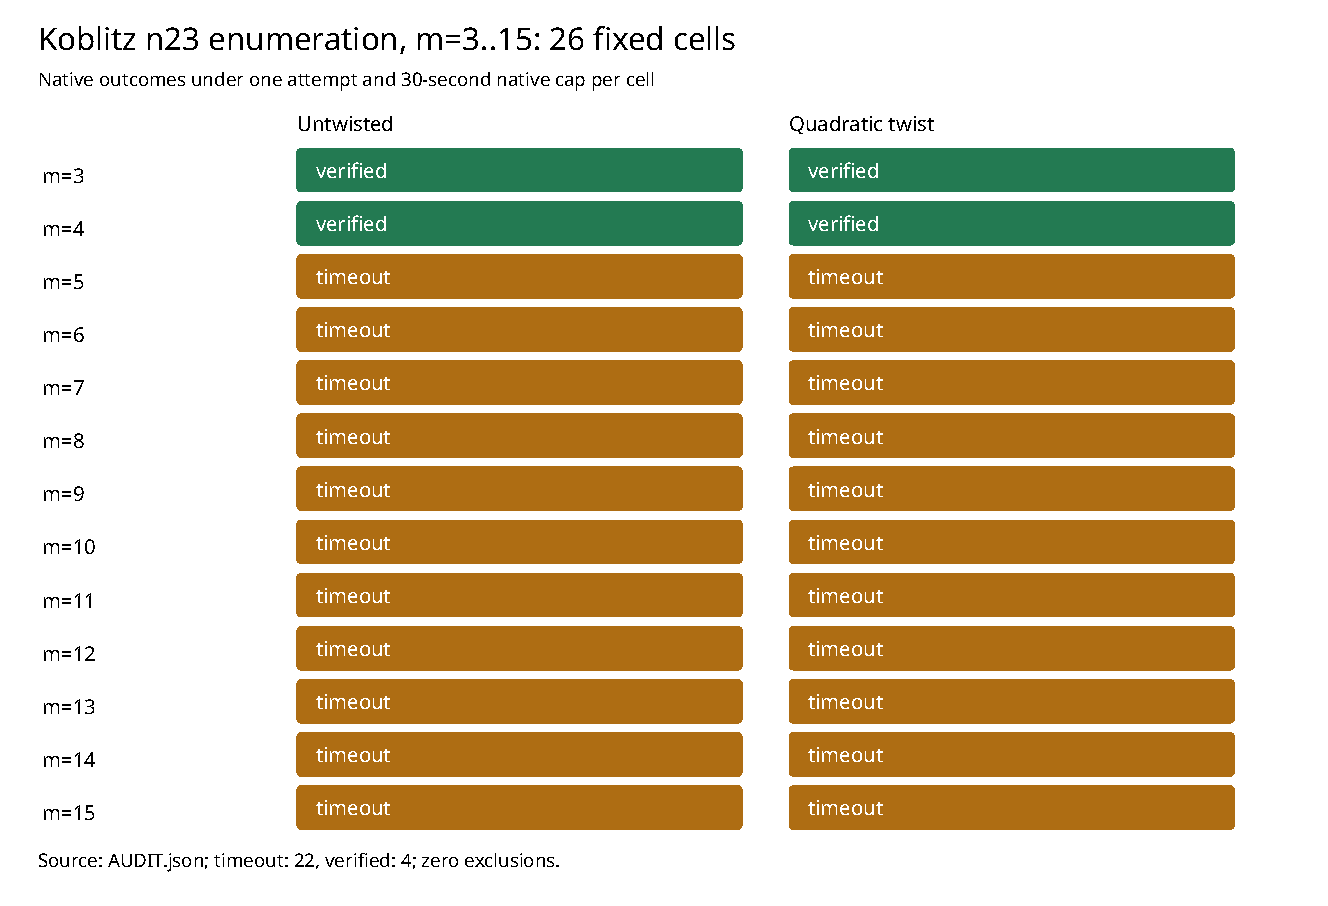
\includegraphics[width=0.92\linewidth]{outcomes.pdf}\end{center}

\subsection*{Exact evidence and measurement scope}
The pinned official export checker accepted 26 planned and attempted rows,
four completed and 22 timed out, with zero exclusions. The independent audit
rehashed 26 archives totaling 8,849,802 bytes and 685 native artifacts;
it checked curve and twist certificates, coefficient-field degree one,
and the matched public input at each arity. The completed m3 cells recorded
512 complete candidates and 584 group-add calls apiece; the completed m4
cells recorded 4,096 and 4,680, respectively.

Eighty-two phase telemetry records are retained, but zero whole-worker
instruction labels qualify for training. An unrelated release compile was
observed during later cells, so timeouts remain resource-conditioned; no
timing-effect comparison is made. Index 18 had one sealed native attempt and
an interrupted pointer client. Fresh S3 reads proved both content-addressed
objects already existed; custody was completed without another PUT or trial.
See \texttt{report/run.md} for hashes, exact receipts and controller amendment.
\end{document}
